%%%%%%%%%%%%%%%%%%%%%%%%%%%%%%%%%%%%%%%%%
% Tecnológico de Costa Rica/Instructivo de Laboratorio de Instrumentación I
% LaTeX Template
% Version 3.1 (25/3/14)
%
% This template has been downloaded from:
% http://www.LaTeXTemplates.com
%
% Original author:
% Linux and Unix Users Group at Virginia Tech Wiki 
% (https://vtluug.org/wiki/Example_LaTeX_chem_lab_report)
%
% License:
% CC BY-NC-SA 3.0 (http://creativecommons.org/licenses/by-nc-sa/3.0/)
%
%%%%%%%%%%%%%%%%%%%%%%%%%%%%%%%%%%%%%%%%%

%----------------------------------------------------------------------------------------
%	PACKAGES AND DOCUMENT CONFIGURATIONS
%----------------------------------------------------------------------------------------

\documentclass[12pt,letterpaper]{report}
\usepackage{amsmath}
\usepackage{amssymb}
\usepackage{siunitx}
\usepackage{float}
\usepackage{tikz}
\def\checkmark{\tikz\fill[scale=0.4](0,.35) -- (.25,0) -- (1,.7) -- (.25,.15) -- cycle;} 
\usepackage{url}
\usepackage[siunitx,american,RPvoltages]{circuitikz}
\ctikzset{capacitors/scale=0.7}
\ctikzset{diodes/scale=0.7}
\usepackage{tabularx}
\newcolumntype{C}{>{\centering\arraybackslash}X}
\renewcommand\tabularxcolumn[1]{m{#1}}% for vertical centering text in X column
\usepackage{tabu}
\usepackage[spanish,es-tabla,activeacute]{babel}
\usepackage{babelbib}
\usepackage{booktabs}
\usepackage{pgfplots}
\usepackage{hyperref}
\hypersetup{colorlinks = true,
            linkcolor = black,
            urlcolor  = blue,
            citecolor = blue,
            anchorcolor = blue}
\usepgfplotslibrary{units, fillbetween} 
\pgfplotsset{compat=1.16}
\usepackage{bm}
\usetikzlibrary{arrows, arrows.meta, shapes, 3d, perspective, positioning,mindmap,trees,backgrounds}
\renewcommand{\sin}{\sen} %change from sin to sen
\usepackage{bohr}
\setbohr{distribution-method = quantum,insert-missing = true}
\usepackage{elements}
\usepackage{verbatim}
\usepackage[edges]{forest}
\usepackage{etoolbox}
\usepackage{schemata}
\usepackage{appendix}
\usepackage{listings}

\definecolor{color_mate}{RGB}{255,255,128}
\definecolor{color_plas}{RGB}{255,128,255}
\definecolor{color_text}{RGB}{128,255,255}
\definecolor{color_petr}{RGB}{255,192,192}
\definecolor{color_made}{RGB}{192,255,192}
\definecolor{color_meta}{RGB}{192,192,255}
\newcommand\diagram[2]{\schema{\schemabox{#1}}{\schemabox{#2}}}

\definecolor{codegreen}{rgb}{0,0.6,0}
\definecolor{codegray}{rgb}{0.5,0.5,0.5}
\definecolor{codepurple}{rgb}{0.58,0,0.82}
\definecolor{backcolour}{rgb}{0.95,0.95,0.92}

\lstdefinestyle{mystyle}{
    backgroundcolor=\color{backcolour},   
    commentstyle=\color{codegreen},
    keywordstyle=\color{magenta},
    numberstyle=\tiny\color{codegray},
    stringstyle=\color{codepurple},
    basicstyle=\ttfamily\footnotesize,
    breakatwhitespace=false,         
    breaklines=true,                 
    captionpos=b,                    
    keepspaces=true,                 
    numbers=left,                    
    numbersep=5pt,                  
    showspaces=false,                
    showstringspaces=false,
    showtabs=false,                  
    tabsize=2
}

\lstset{style=mystyle}
\usepackage{csvsimple}
\usepackage{geometry} 
\geometry{left=18mm,right=18mm,top=21mm,bottom=21mm,headheight=15pt}

\setlength\parindent{0pt} % Removes all indentation from paragraphs

\renewcommand{\labelenumi}{\alph{enumi}.} % Make numbering in the enumerate environment by letter rather than number (e.g. section 6)
\usepackage{fancyhdr}
\pagestyle{fancy}

%----------------------------------------------------------------------------------------
\lhead{Instructivo de Laboratorio de Instrumentación I}
\rhead{\begin{picture}(0,0) \put(-60,0){
\includegraphics[width=20mm]{fig/logo.png}} \end{picture}}
\newcommand{\obj}{Objetivos}
\newcommand{\mat}{Materiales y equipo}
\newcommand{\pro}{Procedimiento}
\newcommand{\capacidad}{Al finalizar este laboratorio el estudiante estará en capacidad de:}
\newcommand{\antesde}{Antes de empezar el laboratorio presente el siguiente cuestionario lleno.}
%----------------------------------------------------------------------------------------
%	DOCUMENT INFORMATION
%----------------------------------------------------------------------------------------


\addto\captionsspanish{\renewcommand{\chaptername}{Laboratorio}}
\addto\captionsspanish{\renewcommand{\tablename}{Tabla}}
\begin{document}


\begin{titlepage}

\begin{center}
\vspace*{1in}
\begin{figure}[htb]
\begin{center}

\includegraphics[width=11cm]{fig/logo.png}
\end{center}
\end{figure}
\vspace*{0.4in}
\begin{Large}
Escuela de Física\\
\vspace*{0.15in}
Ingeniería Física\\
\vspace*{0.8in}
\end{Large}
\vspace*{0.2in}
\begin{Large}
\textbf{Instructivo de Laboratorio} \\
\end{Large}
\vspace*{0.3in}
\begin{large}
Instrumentación I\\
\end{large}
\vspace*{2.5in}
\begin{Large}
\textbf{\today}\\
Versión: 0.1\\
\end{Large}
\rule{80mm}{0.1mm}\\
\vspace*{0.1in}
\begin{large}
Realizado por: Juan J. Rojas y Hugo Sanchez Ortiz\\
\end{large}
\end{center}

\end{titlepage}

\tableofcontents

\chapter{Caracteristicas generales de instrumentos}
\section{\obj}
\capacidad
\begin{itemize}
\item Utilizar la fuente de tensión en voltaje continuo.
\item Utilizar un registrador para tomar datos de sensores.
\item Utilizar sensores para medir corriente y voltaje.
\item Aplicar los conocimientos relacionados a los instrumentos de medición, para el cálculo de valores tales como: exactitud, precisión, error porcentual, desviación estándar, incertidumbre, repetibilidad.
\end{itemize}

\section{\mat}
\begin{itemize}
\item 1 fuente de corriente continua
\item 1 interfaz ScienceWorkshop \textregistered\, 750
\item 1 sensor de corriente CI-6556
\item 1 sensor de voltaje UI-5100
\end{itemize}


\section{\pro}
\begin{enumerate}
\item Realice las conexiones del circuito tal y como se indica en la Figura \ref{fig:L1F1}.

\begin{figure}[H]
    \centering
    \begin{circuitikz} 
        \draw
        (0,0) 	
            to[V, l=$V_f$] 
        (0,4)
        	to[short] 
        (3,4)
        	to[rmeter, t=A]
        (3,2) 
            to[R, l=$R_{sh}$]
        (3,0)-- (0,0)
        (3,4) -- (5,4)
            to[rmeter, t=V] 
        (5,0) -- (3,0)
        ;
    \end{circuitikz}
    \caption{Medición de corriente y voltaje en un circuito.}
    \label{fig:L1F1}
\end{figure}
    
\begin{table}[H]
    \centering
    \caption{Mediciones tomadas a una frecuencia de \SI{1}{\hertz}}
    \vspace{0.5cm}
    \begin{tabular}{ccc}%
    \toprule
    \bfseries &  \multicolumn{2}{c}{\textbf{corrida 1}} \\
    \bfseries tiempo & \bfseries corriente & \bfseries voltaje \\
    {[\si{\second}]} & [\si{\ampere}] & [\si{\volt}]\\
    %\[\si{\second}\] & \[\si{\ampere}\] & \[\si{\volt}\] \\
    \midrule
    \csvreader[
        late after line=\\,
        late after last line=,
        before reading={\catcode`\#=12},
        after reading={\catcode`\#=6}]%
        {data.csv}{1=\time1,2=\current1,3=\voltage1}{\time1 &\current1 & \voltage1}\\
        \bottomrule
    \end{tabular}
    \label{tab:datos}
\end{table}




\item Encienda el interruptor principal de la fuente y gire la perilla principal que permite un voltaje de \SI{10}{\volt}. 
\item La resistencia posee 3 interruptores, accionar el interruptor del centro (600 ohmios). Medir la corriente que circula por la  resistencia y el voltaje que cae en éste, anote el resultado en la Tabla \ref{tab:L1T1}.
\item	Repita las mediciones utilizando los valores de voltaje que indica la Tabla \ref{fig:L1F1} y complete la misma, una vez finalizado la toma de todos los datos, colocar en interruptor principal en OFF. 
\item Calcule indirectamente (Ley de Ohm) para cada caso el valor de la resistencia interna.
\item	Grafique el comportamiento de la resistencia interna y analice los datos obtenidos. 
\item	Cambie ahora el interruptor de la resistencia (300 ohmios), repita los pasos anteriores empezando con cero voltios en la fuente, llene la Tabla \ref{tab:L1T2}.
\item  Grafique el comportamiento de la resistencia y analice el datos obtenidos. 
\item Realice las conexiones del circuito tal y como se indica en la Figura \ref{fig:L1F2}.
\item Encienda el interruptor principal de la fuente y ajuste la tensión a un valor de \SI{100}{\volt}.
\item Realice las mediciones de $I$, $V_{R1}$, $V_{R2}$, $V_{R3}$. Usar un solo amperímetro para medir la corriente, cambiar el otro tester para medir cada tensión. Antes de cambiar la ubicación del medidor de voltaje, colocar el interruptor principal de la fuente en OFF.
\item Tomar como referencia y valores teóricos cada resistencia (1200 ohmios, 600 ohmios y 300 ohmios) según se muestra en el módulo N 8311.
\item Llene la Tabla \ref{tab:L1T3}
\item Realice las conexiones del circuito tal y como se indica en la Figura \ref{fig:L1F3}.

\begin{figure}[H]
\centering
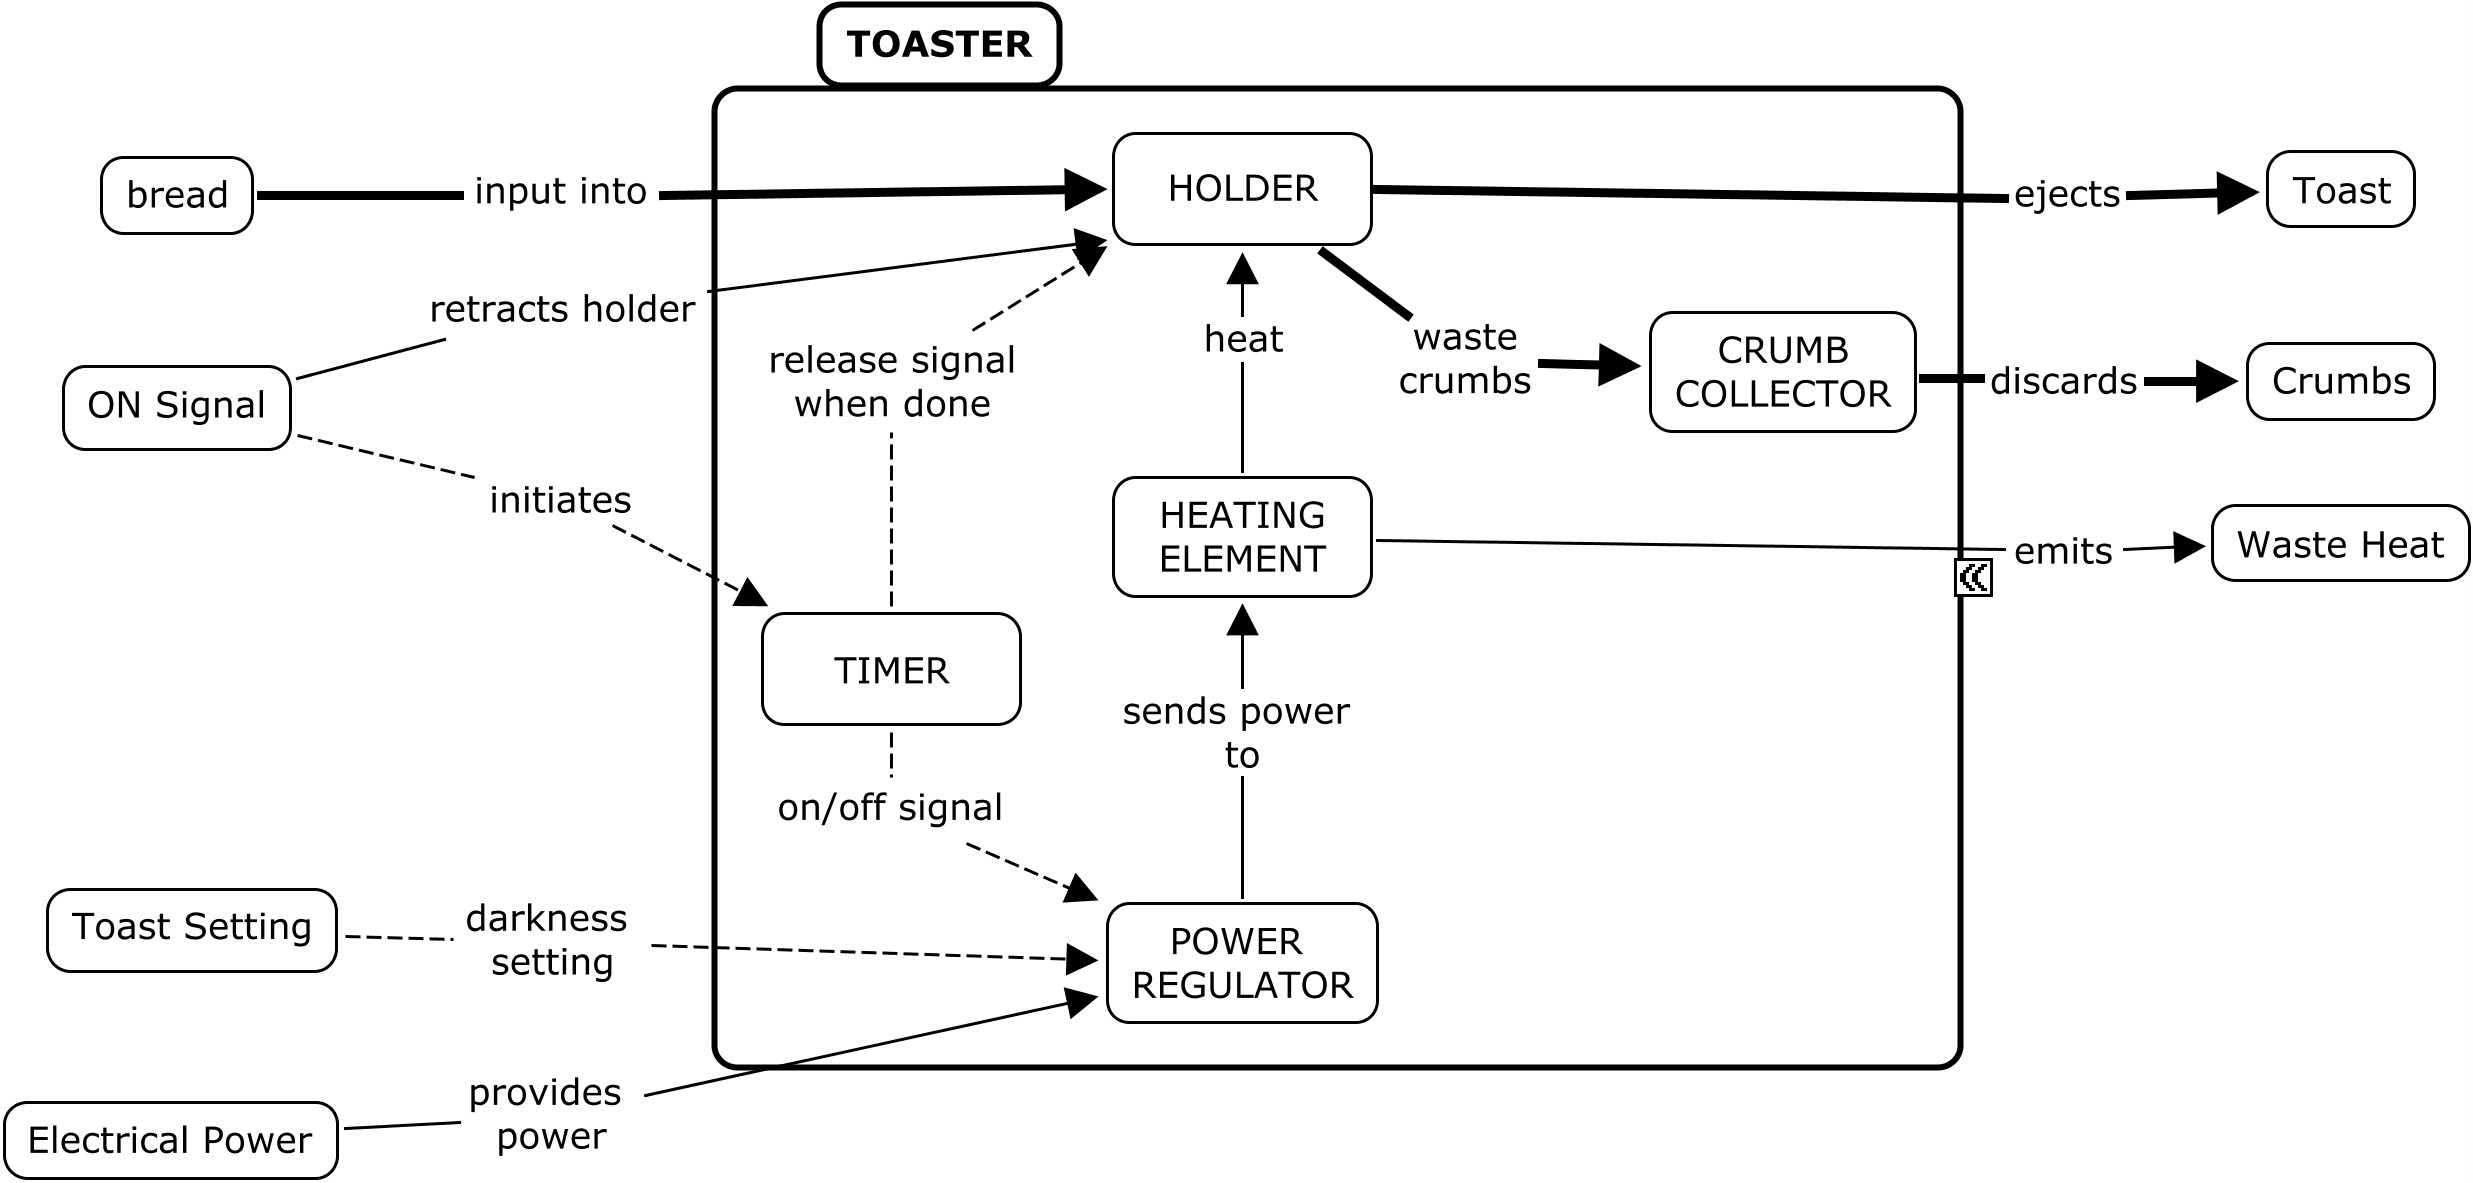
\includegraphics[width=0.5\textwidth]{fig/tostadora.jpg}
\caption{Circuito en Labvolt}
\end{figure}

\item Encienda el interruptor principal de la fuente y ajustar la tensión con un voltaje de \SI{100}{\volt}.
\item Realice las mediciones de $V$, $I_{R1}$, $I_{R2}$, $I_{R3}$.
\item Averigüe los valores teóricos de las resistencias usando el código de colores. 
\item Llene la Tabla \ref{tab:L1T4}
\end{enumerate}

\begin{figure}[H]
\centering
\begin{circuitikz} 
\draw
(0,0) 	
    to[V, l=\SI{100}{\volt}, i=$I$] 
(0,3)
	to[R, l=$R_1$, v=$V_{R1}$] 
(3,3)
	to[R, l=$R_2$, v=$V_{R2}$] 
(6,3) 
    to[R, l=$R_3$, v=$V_{R3}$] 
(9,3) -- (9,0) -- (0,0)
;
\end{circuitikz}
\caption{Circuito en serie con tres resistencias}
\label{fig:L1F2}
\end{figure}

\begin{figure}[H]
\centering
\begin{circuitikz} 
\draw
(0,0) 	
    to[V, l=\SI{100}{\volt}] 
(0,3)
	to[short] 
(2,3)
	to[R, l=$R_1$, i=$I_{R1}$] 
(2,0)
    --
(0,0)
(2,3)
    --
(4,3)
    to[R, l=$R_2$, i=$I_{R2}$] 
(4,0)
    --
(2,0)
(4,3)
    --
(6,3)
    to[R, l=$R_3$, i=$I_{R3}$]
(6,0)
    --
(4,0)
;
\end{circuitikz}
\caption{Circuito en paralelo con tres resistencias}
\label{fig:L1F3}
\end{figure}

\begin{table}[H]
	\caption{Valores experimentales de corriente y voltaje 600 ohmios}
	\label{tab:L1T1}
	\centering
	\vspace{0.5cm}
	\begin{tabularx}{6cm}{CCC}
		\toprule
		$V_B$ (\si{V}) & $I_B$(\si{\ampere}) & $R_B$($\Omega$)\\
		\midrule
		0 & & \\
		10 & & \\
		20 & & \\
		30 & & \\
		40 & & \\
		50 & & \\
		60 & & \\
		70 & & \\
		80 & & \\
		90 & & \\
		100 & & \\	
		
		\bottomrule
	\end{tabularx}
\end{table}
\begin{table}[H]
	\caption{Valores experimentales de corriente y voltaje 300 ohmios}
	\label{tab:L1T2}
	\centering
	\vspace{0.5cm}
    \begin{tabularx}{6cm}{CCC}
		\toprule
		$V_R$ (\si{V}) & $I_R$(\si{\ampere}) & R($\Omega$)\\
		\midrule
		0 & & \\
		10 & & \\
		20 & & \\
		30 & & \\
		40 & & \\
		50 & & \\
		60 & & \\
		70 & & \\
		80 & & \\
		90 & & \\
		100 & & \\
		\bottomrule
	\end{tabularx}
\end{table}

\begin{table}[H]
	\caption{Método indirecto de la ley de Ohm aplicado en un circuito con tres resistencias en serie}
	\label{tab:L1T3}
	\centering
	\vspace{0.5cm}
    \begin{tabularx}{14cm}{CCCCCC}
		\toprule
		& $V$ (\si{V}) & $I$(\si{\milli\ampere}) & $R_{teor}$(\si{\ohm}) & $R_{exp}$(\si{\ohm}) & error (\%)\\
		\midrule
		$R_1$ & & &1200 & & \\
		$R_2$ & & &600 & & \\
		$R_3$ & & &300 & & \\
		\bottomrule
	\end{tabularx}
\end{table}

\begin{table}[H]
	\caption{Método indirecto de la ley de Ohm aplicado en un circuito con tres resistencias en paralelo}
	\label{tab:L1T4}
	\centering
	\vspace{0.5cm}
    \begin{tabularx}{14cm}{CCCCCC}
		\toprule
		&$V$ (\si{V}) & $I$(\si{\milli\ampere}) & $R_{teor}$(\si{\ohm}) & $R_{exp}$(\si{\ohm}) & error (\%)\\
		\midrule
	    $R_1$ & & &1200 & & \\
		$R_2$ & & &600 & & \\
		$R_3$ & & &300 & & \\
		\bottomrule
	\end{tabularx}
\end{table}


\appendix
\chapter{El osciloscopio digital}
\label{ap:osc}
\section{Introducción.} La naturaleza se mueve de manera sinusoidal; véase el movimiento de las olas, los terremotos, el sonido a través de aire o la frecuencia natural de un cuerpo en movimiento. Incluso la luz (parte partícula, parte onda) tiene una frecuencia fundamental, la cual se puede observar a través del color. Los sensores pueden convertir estas fuerzas en señales eléctricas que se pueden observar y estudiar con el osciloscopio.\\
Es por esto que el osciloscopio es una herramienta indispensable para cualquiera que esté diseñando, manufacturando o reparando algún dispositivo electrónico, es la clave para conocer los retos demandantes de la medición en la actualidad. Con el sensor correcto, un osciloscopio puede medir todo tipo de fenómenos debido a que un sensor crea una señal eléctrica en respuesta de un estímulo físico, como el sonido, esfuerzo mecánico, presión, luz, o calor.\\
Los conceptos presentados en este apéndice darán una línea base para entender operaciones y funciones básicas del osciloscopio.
\section{El osciloscopio.} El osciloscopio básicamente es un dispositivo de gráfica y muestra de datos, este proyecta un gráfico de una señal eléctrica. En la mayoría de las aplicaciones este gráfico demuestra como las señales cambian en el tiempo: el eje de las ordenadas (Y) representa el voltaje y el eje de las abscisas (X) representa el tiempo. Además, se dice que el eje Z representa la intensidad o el brillo del monitor.\\
Este simple gráfico puede dar muchísima información valiosa, por ejemplo: los valores de voltaje y tiempo de la señal, la frecuencia de oscilación, las partes móviles de un circuito representados en una señal, la frecuencia a la cual una porción de la señal está ocurriendo relativa a otras porciones, si un componente está o no distorsionando la señal, que tanto una señal es de corriente directa o que tanto es de corriente alterna, que porción de la señal es ruido o como cambia el ruido en función del tiempo.\\
Los osciloscopios se pueden clasificar en dos: analógicos y digitales. A su vez los osciloscopios digitales pueden ser de almacenamiento digital (DSO), de fósforo digital (DPO) u osciloscopios de muestreo.
\subsection{El osciloscopio de almacenamiento digital.} El osciloscopio digital, a diferencia del analógico, utiliza un convertidor analógico-digital (ADC) el cual convierte las mediciones de voltaje en señales digitales de información. Este adquiere la forma de la señal como una serie de muestreos y los guarda hasta acumular los suficientes para poder describir la forma de onda.\\
Los osciloscopios de almacenamiento digital tienen la cualidad de que pueden capturar y ver eventos que posiblemente solo ocurren una vez, comúnmente llamados transientes. Esto debido a que la información de la onda existe de manera digital, como una serie de valores binarios, lo cual permite que sean analizados, impresos, procesados y archivados.
\subsection{Señales eléctricas.} Debido a que lo que el propósito principal el osciloscopio es de proyectar señales eléctricas, es importante entender los conceptos básicos de las mismas.
\begin{itemize}
\item \textbf{Amplitud.} Las dos definiciones comúnmente utilizadas por los ingenieros son la amplitud pico y la amplitud RMS. El valor pico es la magnitud máxima de la señal, el valor RMS se calcula elevando al cuadrado la señal, se encuentra su valor promedio y se le saca la raíz cuadrada a este valor.
\item \textbf{Desfase} Se refiera a la cantidad de translación horizontal entre dos señales, se mide en grados o en radianes. Para una forma de onda sinusoidal, un ciclo se presenta como 360$^{\circ}$, por lo tanto, si dos señales sinusoidales se difieren por medio ciclo, su desfase es de 180$^{\circ}$.
\item \textbf{Periodo} Es el tiempo en el cual la forma de onda se repite, el tiempo en el que cumple un ciclo, se mide en segundos.
\item \textbf{Frecuencia.} Es el número de veces que una onda se repite en un segundo, es el recíproco del periodo y se mide en Hertz.
\item \textbf{Tipos de onda.} Existe varios tipos de onda, las más comunes son las sinusoidales, rectangulares o cuadradas, triangulares o diente sierra y los pulsos.
\item\textbf{Señales analógicas y digitales} Las señales analógicas son capaces de tener cualquier valor dentro de un rango en el tiempo, las señales digitales son discretas, típicamente tienen solo dos posibles valores (High o Low, 1 o 0, 5V o 0V)
\end{itemize}
\subsection{Integridad de la señal.} La integridad de la señal es la habilidad del osciloscopio para reconstruir la forma de onda de manera precisa. Para definir la integridad de la señal es necesario responder las siguientes preguntas: ¿es la señal proyectada, verdaderamente la señal que ocurre? ¿La forma de onda está clara o se ve distorsionada? ¿Cuántas tomas de señal se pueden obtener por segundo? La integridad de la señal es de suma importancia ya que es inútil desarrollar una prueba donde la forma de onda en el osciloscopio no posee la misma forma o características de la verdadera señal.
\subsection{Sistemas y controles de un osciloscopio.} La mayoría de los osciloscopios están compuestos por cuatros sistemas. El sistema vertical, el sistema horizontal, el sistema de disparo y el sistema de visualización. Conocer el funcionamiento de cada uno de estos sistemas y controles le permitirán reconstruir de manera precisa la señal estudiada manteniendo así la integridad de esta.\\
Cuanto se utiliza un osciloscopio, es necesario ajustar tres comandos básicos para acomodar la señal de entrada: Primero la atenuación o amplitud de la señal, utilizando el control volts/div para ajustar la amplitud de la señal al rango deseado. Segundo la base del tiempo, para esto se utiliza el control sec/div, esto permite ajustar la cantidad de tiempo por división representada en el eje horizontal de la pantalla. Tercero, el “trigger” o disparo del osciloscopio el cual tiene la función de estabilizar una señal repetitiva.\\
Buenas prácticas, antes de iniciar las mediciones, son: Verificar que el canal de entrada que se está utilizando está encendido. Presionar, si se posee, el botón [Default Settings] esto ajustará el osciloscopio a su configuración predeterminada. Seguidamente presionar, si se posee, el botón [Autoscale] esto va a ajustar automáticamente la escala vertical y horizontal para que la señal se pueda ver de una manera clara en la pantalla. Estas recomendaciones también son útiles cuando se ha perdido la señal de la onda y no se puede proyectar bien en el osciloscopio.

\subsubsection{Sistema vertical y controles.} Se utiliza para posicionar y escalar la forma de onda verticalmente, además se utiliza para ajustar el acoplamiento de entrada y otras condiciones de la señal.
\begin{itemize}
\item \textbf{Posición y volts/div: } El control de posición vertical permite mover la forma de onda hacia arriba y abajo justo donde se desee en la pantalla. El control volt/div varía el tamaño de la forma de onda en la pantalla. Se puede ver como un factor de escala por lo tanto el máximo voltaje que se puede proyectar es los volts/div multiplicado por el número de divisiones verticales.
\item \textbf{Límite de ancho de banda:} La mayoría de los osciloscopios tienen un circuito que limita el ancho de banda. Esto permite reducir el ruido que algunas veces puede aparecer en la forma de onda, produciendo así una señal más clara.
\end{itemize}
\subsubsection{Sistema horizontal y controles.} Este sistema está más relacionado con la adquisición de la señal de entrada y la frecuencia de muestreo. Los controles se utilizan para posicionar y escalar la forma de onda de manera horizontal.
\begin{itemize}
\item \textbf{Modos de adquisición:} Los modos de adquisición controlan como se producen los puntos de muestreo de la forma de onda. Estos puntos son los valores digitales que derivan directamente del convertidor ADC. El intervalo de muestreo se refiere al tiempo entre cada punto de muestreo. Puntos de la forma de onda son los valores digitales que son guardados en la memoria y proyectados para construir la señal. Los tipos de modos de adquisición son: Modo de muestreo, modo de detección pico, modo de alta resolución, modo envolvente, modo promedio.
\item \textbf{Métodos de muestreo:} Existen diferentes métodos de implementar tecnologías de muestreo, sin embargo, en la actualidad los métodos más utilizados son el muestreo de tiempo real y el muestreo de tiempo equivalente.\\
El muestreo de tiempo real es ideal para señales cuyo rango de frecuencia es menos que la mitad de la frecuencia de muestreo máxima del osciloscopio. Aquí el osciloscopio puede adquirir suficientes puntos en el barrido de la forma de onda, construyendo así una imagen clara y manteniendo la integridad de la señal. Esta es la única forma de capturar transientes rápidos en la señal con un osciloscopio digital.\\
El muestro de tiempo equivalente es utilizado cuando la frecuencia de la señal es mayor a la mitad de la frecuencia de muestreo del osciloscopio. Esto debido a que, a frecuencias altas, el osciloscopio puede no estar habilitado para recolectar suficientes muestras en un barrido. Este método toma ventaja del hecho de que la mayoría de las ocurrencias, naturales y creadas por el humano, son eventos repetitivos; por lo tanto, construye una imagen de una señal repetitiva capturando un poco de información de cada repetición.
\item \textbf{Posición y sec/div:} La posición horizontal mueve la forma de onda hacia la izquierda o derecha, exactamente donde se desee. Ajustar los sec/divs permite seleccionar la velocidad a la cual la forma de onda se proyectará a lo largo de la pantalla. Esto es un factor de escala y cambiar los sec/div permite observar mayores o menores intervalos de tiempo de la señal de entrada.
\item \textbf{Modos XY:} La mayoría de los osciloscopios tiene el modo XY, este permite proyectar, en el eje horizontal, una señal de entrada en lugar de una basada en el tiempo. Esto tiene varias aplicaciones prácticas.
\end{itemize}
\subsubsection{Sistemas y controles de disparo.} Esta función ayuda a sincronizar el barrido horizontal al punto correcto de la señal, esencialmente para aclarar las características de esta. Ayuda a estabilizar las formas de onda repetitivas y capturar así una señal estática, esto es posible por la proyección repetida de la misma porción de la señal. Esta función es importante ya que permite que esta porción de la señal sea utilizable, analizable y entendible. Los tipos de disparo más comunes son:
\begin{itemize}
\item \textbf{Disparo de flanco:} Es el modo de disparo más utilizado. El disparo ocurre cuando el voltaje sobrepasa un valor umbral establecido. Se puede escoger el disparo en el flanco positivo o en el flanco negativo
\item \textbf{Disparo por falla:} Este modo permite que se dispare en un evento o pulso cuyo ancho es mayor o menor que un período de tiempo especificado. Esta capacidad es muy útil para encontrar fallas o errores aleatorios.
\item \textbf{Disparo por ancho de pulso:} Es similar al disparo por falla, sin embargo, es más general en el sentido de que se puede disparar los pulsos en un ancho específico y se puede escoger la polaridad (positiva o negativa) de los pulsos a disparar. Además se puede ajustar la posición horizontal del disparo.
\end{itemize}
\section{Funciones matemáticas básicas.} Adicionalmente a las funciones anteriormente descritas, la mayoría de los osciloscopios digitales incluyen las siguientes funciones matemáticas.
\begin{itemize}
\item \textbf{Transformada de Fourier.} Permite ver las frecuencias que componen la señal.
\item \textbf{Valor Absoluto.} Esta función matemática muestra el valor absoluto (refiriéndose al voltaje) de la forma de onda.
\item \textbf{Integración.} Esta función matemática calcula el valor de la integral de la forma de onda.
\item \textbf{Suma y resta.} Esta función es útil ya que permite sumar o restar múltiple formas de onda y proyectar el resultado de la forma de onda de la operación. 
\end{itemize}
\textbf{Referencias.} Este apéndice está inspirado en los siguientes documentos:
\begin{itemize}
    \item[[1]] K. Technologies, “Basic Oscilloscope Fundamentals,” 2017 [Online]. Available: www.keysi\\ght.com 
    \item[[2]] Tektronix, “Oscilloscope Fundamentals,” 2009 [Online]. Available: www.tektronix.com
\end{itemize}

%----------------------------------------------------------------------------------------
%	BIBLIOGRAPHY
%----------------------------------------------------------------------------------------

\bibliographystyle{ieeetr}

\bibliography{referencias}

%----------------------------------------------------------------------------------------


\end{document}